%%%%%%%%%%%%%%%%%%%%%%%%%%%%%%%%%%%%%%%%%%%%%%%%%%%%%%%%%%%%%%%%%%%%%%%%%%%%%%%%
%2345678901234567890123456789012345678901234567890123456789012345678901234567890
%        1         2         3         4         5         6         7         8

\documentclass[letterpaper, 10 pt, conference]{ieeeconf}  % Comment this line out if you need a4paper

%\documentclass[a4paper, 10pt, conference]{ieeeconf}      % Use this line for a4 paper

\IEEEoverridecommandlockouts                              % This command is only needed if 
                                                          % you want to use the \thanks command

\overrideIEEEmargins                                      % Needed to meet printer requirements.

% See the \addtolength command later in the file to balance the column lengths
% on the last page of the document

% The following packages can be found on http:\\www.ctan.org
%\usepackage{graphics} % for pdf, bitmapped graphics files
%\usepackage{epsfig} % for postscript graphics files
%\usepackage{mathptmx} % assumes new font selection scheme installed
%\usepackage{times} % assumes new font selection scheme installed
%\usepackage{amsmath} % assumes amsmath package installed
%\usepackage{amssymb}  % assumes amsmath package installed

\linespread{0.99}

\title{\LARGE \bf
TinyRobo: A Platform for Tabletop Swarm Research
}


\author{Abraham Shultz$^{1}$% <-this % stops a space
%\thanks{*This work was not supported by any organization}% <-this % stops a space
\thanks{$^{1}$Department of Computer Science,
        University of Massachusetts Lowell, 1 University Ave, Lowell, Massachusetts, USA
        {\tt\small ashultz@cs.uml.edu}}%
}

\usepackage{graphicx}
\usepackage{caption}
\usepackage{subcaption}
\usepackage{auto-pst-pdf}
\usepackage{graphviz}
\usepackage{url}
\usepackage{xargs} 
\usepackage[colorinlistoftodos,prependcaption,textsize=tiny]{todonotes}
\newcommandx{\unsure}[2][1=]{\todo[linecolor=red,backgroundcolor=red!25,bordercolor=red,#1]{#2}}
\newcommandx{\change}[2][1=]{\todo[linecolor=blue,backgroundcolor=blue!25,bordercolor=blue,#1]{#2}}
\newcommandx{\info}[2][1=]{\todo[linecolor=OliveGreen,backgroundcolor=OliveGreen!25,bordercolor=OliveGreen,#1]{#2}}
\newcommandx{\improvement}[2][1=]{\todo[linecolor=purple,backgroundcolor=purple!25,bordercolor=purple,#1]{#2}}
\newcommandx{\thiswillnotshow}[2][1=]{\todo[disable,#1]{#2}}

\begin{document}



\maketitle
\thispagestyle{empty}
\pagestyle{empty}


%%%%%%%%%%%%%%%%%%%%%%%%%%%%%%%%%%%%%%%%%%%%%%%%%%%%%%%%%%%%%%%%%%%%%%%%%%%%%%%%
\begin{abstract}

Previous platforms for swarm robotics have relied on custom-manufactured mechanical assemblies for their mobility. Because these assemblies are usually hand-made in limited numbers, they restrict the availability of swarm robots to organizations with large budgets. Recent attempts to avoid this problem, such as the Harvard Kilobots \cite{rubenstein2014kilobot} have reduced sensing and processing ability in order to remain small in size. This paper presents a hardware platform and a proposed software infrastructure to sidestep both problems, resulting in a swarm platform that is cheap and easy for researchers to duplicate. The platform permits heterogeneous mobility solutions and flexible virtualization of sensing and inter-robot networking.   

\end{abstract}


%%%%%%%%%%%%%%%%%%%%%%%%%%%%%%%%%%%%%%%%%%%%%%%%%%%%%%%%%%%%%%%%%%%%%%%%%%%%%%%%
\section{Introduction}

Swarm robots used in research are generally small. 
The reason to keep swarm robots small is at least three-fold. 
First, larger robots consume more materials per unit, and so cost more money.
As a result, for a given number of swarm units, larger robots will result in a higher cost swarm. 
Second, each robot requires some amount of space to move around in. 
To keep the ratio of free space to robots constant, the area of space used by the robots grows as the robots do. 
If the ratio isn't kept constant, the robots will crowd each other, and so large robots will require either a very large space, or become overly crowded. 
The challenge of swarm robot hardware, then, is to put all of the same parts as non-swarm robots: a mobility platform, a power supply, a processor, sensors, and communication hardware, into a small package.

The robots used in most swarm research are of a sufficiently small size that many of them can fit in a room, mostly between 1cm$^3$ and 0.3m$^3$. 
This scale range divides fairly evenly into robots that can operate in large swarms on a table, and those that can operate in swarms within a room, albeit possibly a large room. 
For the purposes of this work, only tabletop swarms are considered. 

\section{Overview of Previous Swarm Hardware}

Tabletop swarm robots generally occupy the size range from 1cm$^3$ to 15cm$^3$.
Many impressive designs for small swarm robot platforms have been proposed and constructed as part of research in swarm robotics. 
At the low end, in terms of scale, the I-SWARM Project was intended to create a 2x2x1mm robot that moved by stick-slip locomotion actuated by piezo levers \cite{seyfried2005swarm}. 
Other techniques have been developed to use magnetic fields to apply force to small magnetic objects, resulting in controlled motion of the objects \cite{pelrine2012diamagnetically}.
Alice \cite{caprari1998autonomous} combined a PIC16F84 processor, motors, RF and IR networking, and enough battery power for 10 hours of autonomy into a robot measuring under 2.5cm$^3$. 
The AmIR robot was similar to Alice in size and capability, but with a more modern processor\cite{arvin2009development}.
The Jasmine swarm robots were possibly the closest approach to a commercially-available successor to Alice \cite{kernbach2011swarmrobot}.
Jasmine measured 26x26x20mm, and included an ATMega processor, IR communication and obstacle detection, two motor skid steering, and li-po batteries.
InsBot was a small robot, measuring 41x30x19mm, that was designed to interact with cockroaches \cite{colot2004insbot}.
It used two processors, one to run higher level behaviors and one to interface with a suite of sensors that included 12 IR sensors and a linear camera. 

None of the previously listed robots are currently commercially available, and many of them never were. 
Even when they are commercially available, most existing swarm robots are too expensive to build a large swarm.
The Epuck from EFPL costs approximately 800 Swiss francs (\$810 USD) per unit, so the cost of maintaining a large swarm can become daunting quickly. 
Jasmine robots cost about 100 Euro (\$111 USD) when they were available. 
Even the Kilobots \cite{rubenstein2014kilobot} cost 1100 Swiss francs for a 10-pack, or about \$112 (US) per robot. 

One way to reduce the cost of swarm robots is to use commercial, off-the-shelf (COTS) hardware in the construction of the robot. 
Reusing existing hardware leverages the economies of scale that reduce the price of commercial hardware, as well as eliminating the need to design or build the COTS parts. 
Use of COTS parts in research robotics has led to at least two platforms referred to as COTSBots \cite{bergbreiter2003cotsbots, soule2011cotsbots}.
The first COTSBots used mote hardware for the communications link and sensing, plus a motor control add-on board \cite{bergbreiter2003cotsbots}. 
These COTSBots used a specific brand of high-quality micro RC car for mobility.
At the time of this writing, the car used in COTSBots is moderately expensive for a toy car, costing a little over \$100USD per unit. 
 
\section{TinyRobo Hardware}

In order to avoid the sensitivity to the work surface exhibited by the Kilobots and, to a lesser extent, the Epucks, TinyRobo uses children's toys as mobility platforms. 
The TinyRobo controller module replaces the control electronics of the toys, similar to the Spider-Bots developed by Laird, Price, and Raptis or Bergbreiter's COTSBots \cite{lairdspider, bergbreiter2003cotsbots}.
However, unlike the Spider-Bots and COTSBots, TinyRobo does not specify a particular toy chassis to use for mobility. 
TinyRobos are intended to be heterogeneous, partly because of the advantages of heterogeneity in a swarm, and partly because toy supplies are unreliable.
While toys in the general case are expected to remain available, a particular line of toys might be discontinued or a modified version released. 
The software framework in development to support TinyRobos is based on ROS, and so will allow modular replacement of the control algorithms used to convert desired motion of the robot into drive signals for the motors. 

\begin{figure}
	\centering
	\begin{subfigure}{0.22\textwidth}
		\centering
		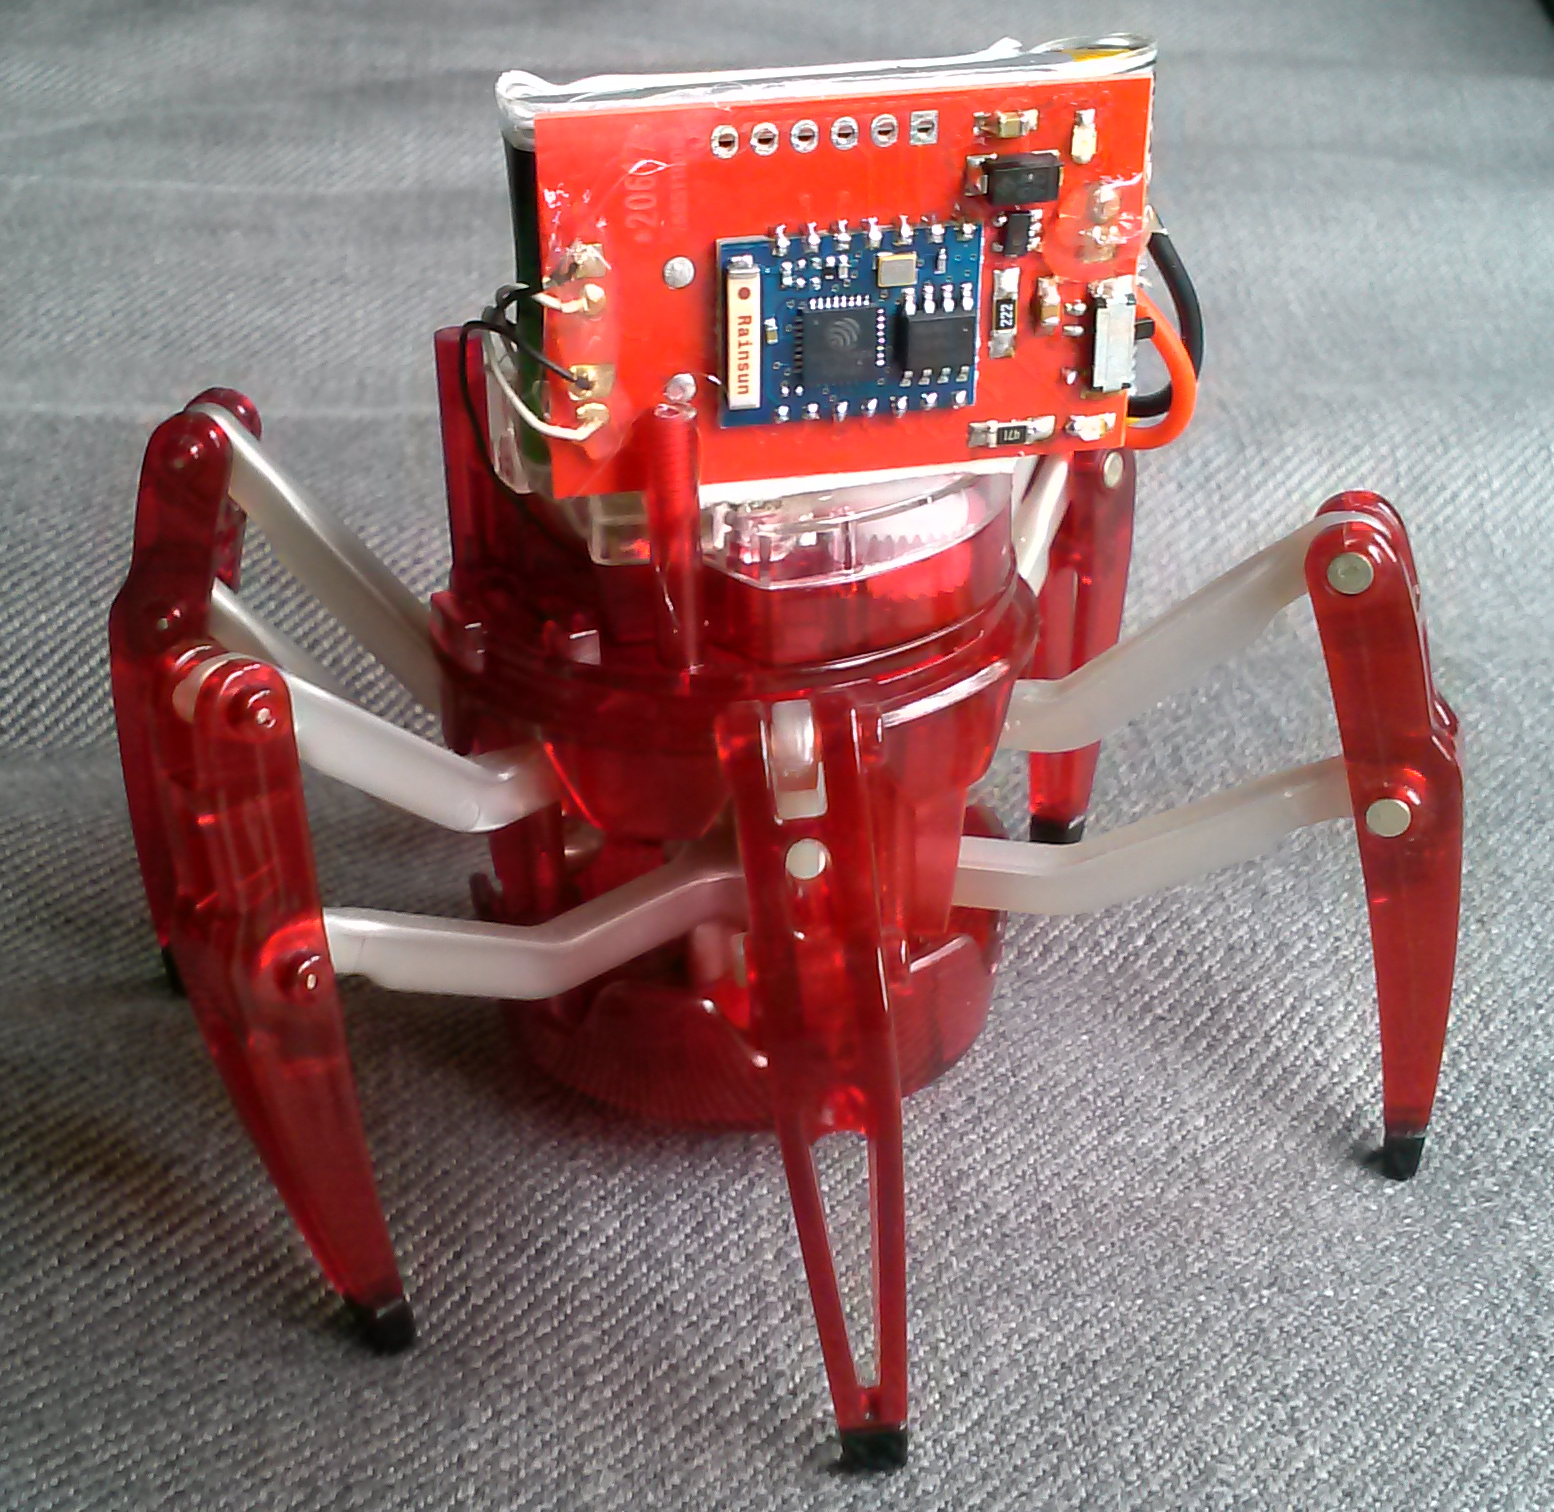
\includegraphics[width=\linewidth]{tiny_spider}
		\caption{Spider base}
		\label{fig:sub1}
	\end{subfigure}%
	\begin{subfigure}{0.22\textwidth}
		\centering
		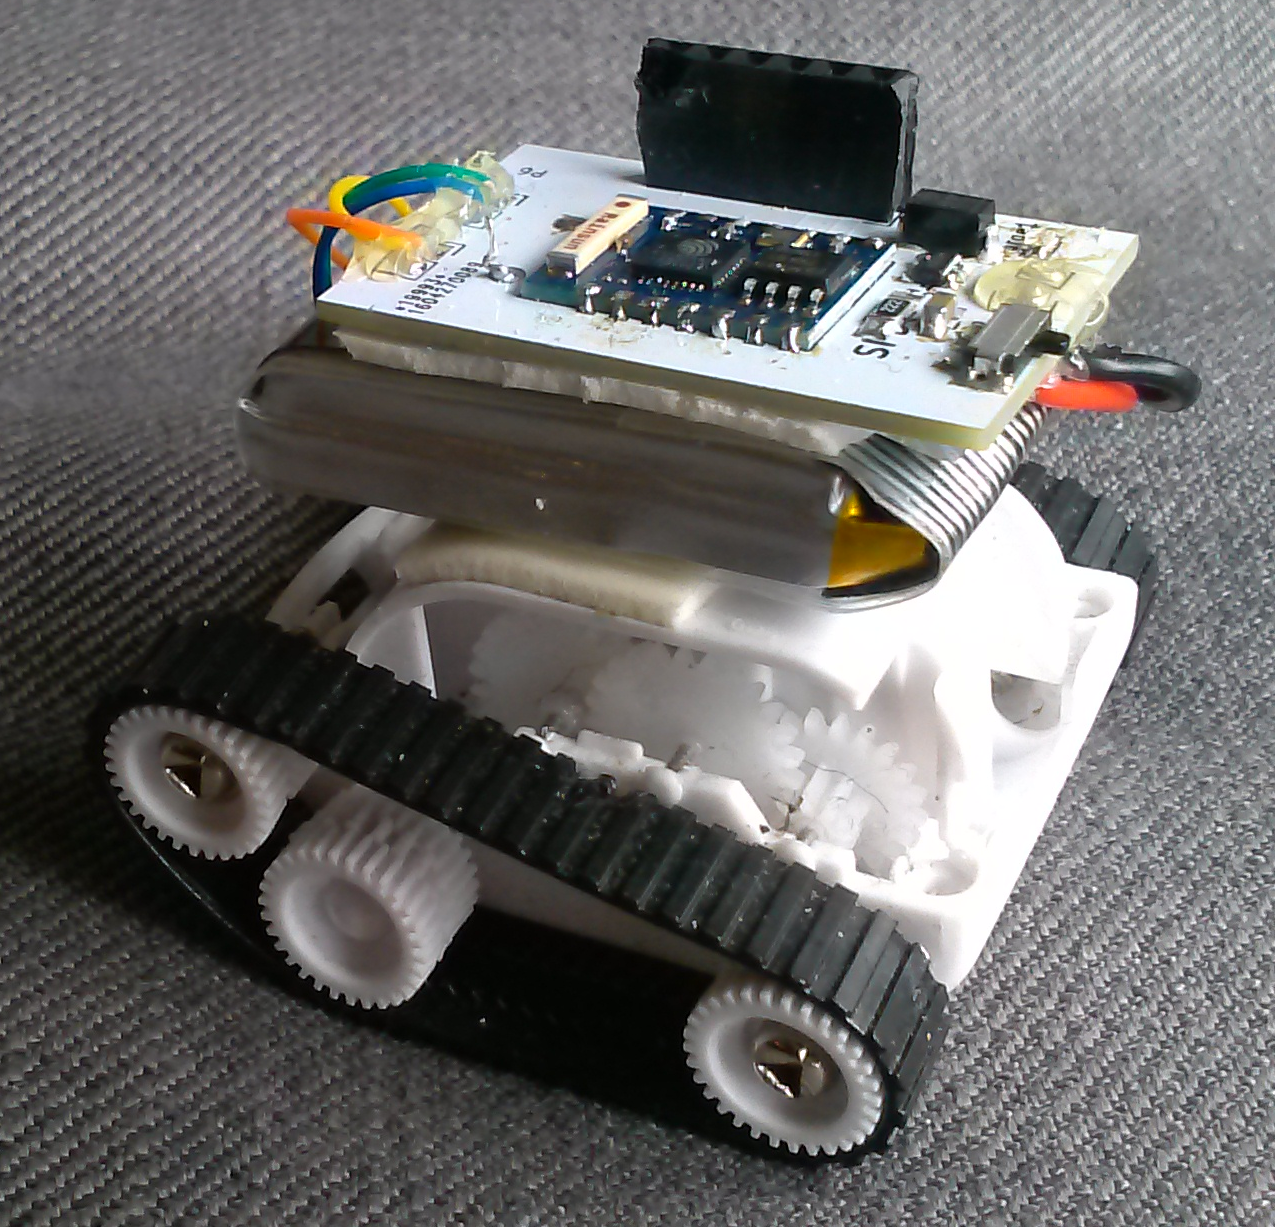
\includegraphics[width=\linewidth]{tiny_tank}
		\caption{Tank-style base}
		\label{fig:sub2}
	\end{subfigure}
	\label{fig:test}
\end{figure}

Most children's toys use either one motor with a mechanical linkage to cause the toy to turn when the motor is reversed, or two motors.
Two-motor toys frequently use either differential steering or have one motor supply drive power and the other provide steering. 
All of these toys can be controlled by TinyRobo controller modules.

The processor of the TinyRobo controller is an ESP-8266 wifi module.
The ESP-8266 costs approximately \$3-5, and contains both a wireless interface and a microcontroller that can be programmed in a variety of languages, including the Arduino variant of C/C++.   
The ESP-8266 is available in several form factors; the version selected is the ESP-8266-03, which provides more GPIO pins than the others, and has an internal antenna.

The motor controller in the TinyRobo boards is the DRV8830 IC by Texas Instruments. 
The DRV8830 provides 1A of drive current, and is controlled by the ESP-8266 over an I2C serial interface. 
Experimental tests with 8 different toys indicate that small toys draw well under 1A while moving freely, and peak around 2A when the motors are stalled. 
The DRV8830 provides overcurrent limiting, so a stall condition or short circuit of the motor leads will disable the motor drive, but not damage the DRV8830. 

The I2C interface used for the motor drivers can be extended to customize the robots, by adding sensors or more motor drivers, but this was not done in this version for cost reasons. 
Future versions of the board may include connection points for I2C expansions, but at present these expansions can be connected to the same traces that provide I2C signals to the motor drivers. 

The TinyRobo control module also provides connections for a 3.7V lithium-ion battery pack, as well as charge control circuitry for the battery. 
The battery is charged by power provided a separate USB-to-serial adapter board, the Sparkfun BOB-11736. 
The USB-to-serial adapter also controls reset and entry into programming mode to change the programming of the TinyRobo controller. 
Moving this functionality to the adapter board reduces the size and cost of the TinyRobo control module. 

Instead of a comprehensive suite of physical sensors, a software framework is being developed to provide virtual sensors based on the view from a camera mounted over the swarm experiment area.
This software framework will also provide virtualized inter-robot networking and computational power beyond that available on the robots. 
As a result, the robots will be able to behave as though they had capabilities such as global localization and obstacle range sensors, without having such hardware on the robots.

\section{Conclusions}

TinyRobo provides a hardware platform for relatively cheap and easy construction of tabletop swarm robots.
Unlike many previously existing platforms, it is commercially available, and can be extended by users to new mobility hardware. 
The TinyRobo schematics and PCB design files are available at \url{https://github.com/ab3nd/TinyRobo/}, and the PCBs are commercially available from Dirty PCBs at  \url{http://dirtypcbs.com/view.php?share=20617&accesskey=775edbb47111a5cd47e422829b761675}

\section{Acknowledgements}

This work was supported in part by the National Science Foundation through IIS-1426968. 

\bibliographystyle{apalike}
\bibliography{rm2.bib}

\end{document}
